\documentclass[border=0.2cm]{standalone}

% Required packages
\usepackage{tikz}
\usetikzlibrary{shapes,positioning}

\begin{document}
	
	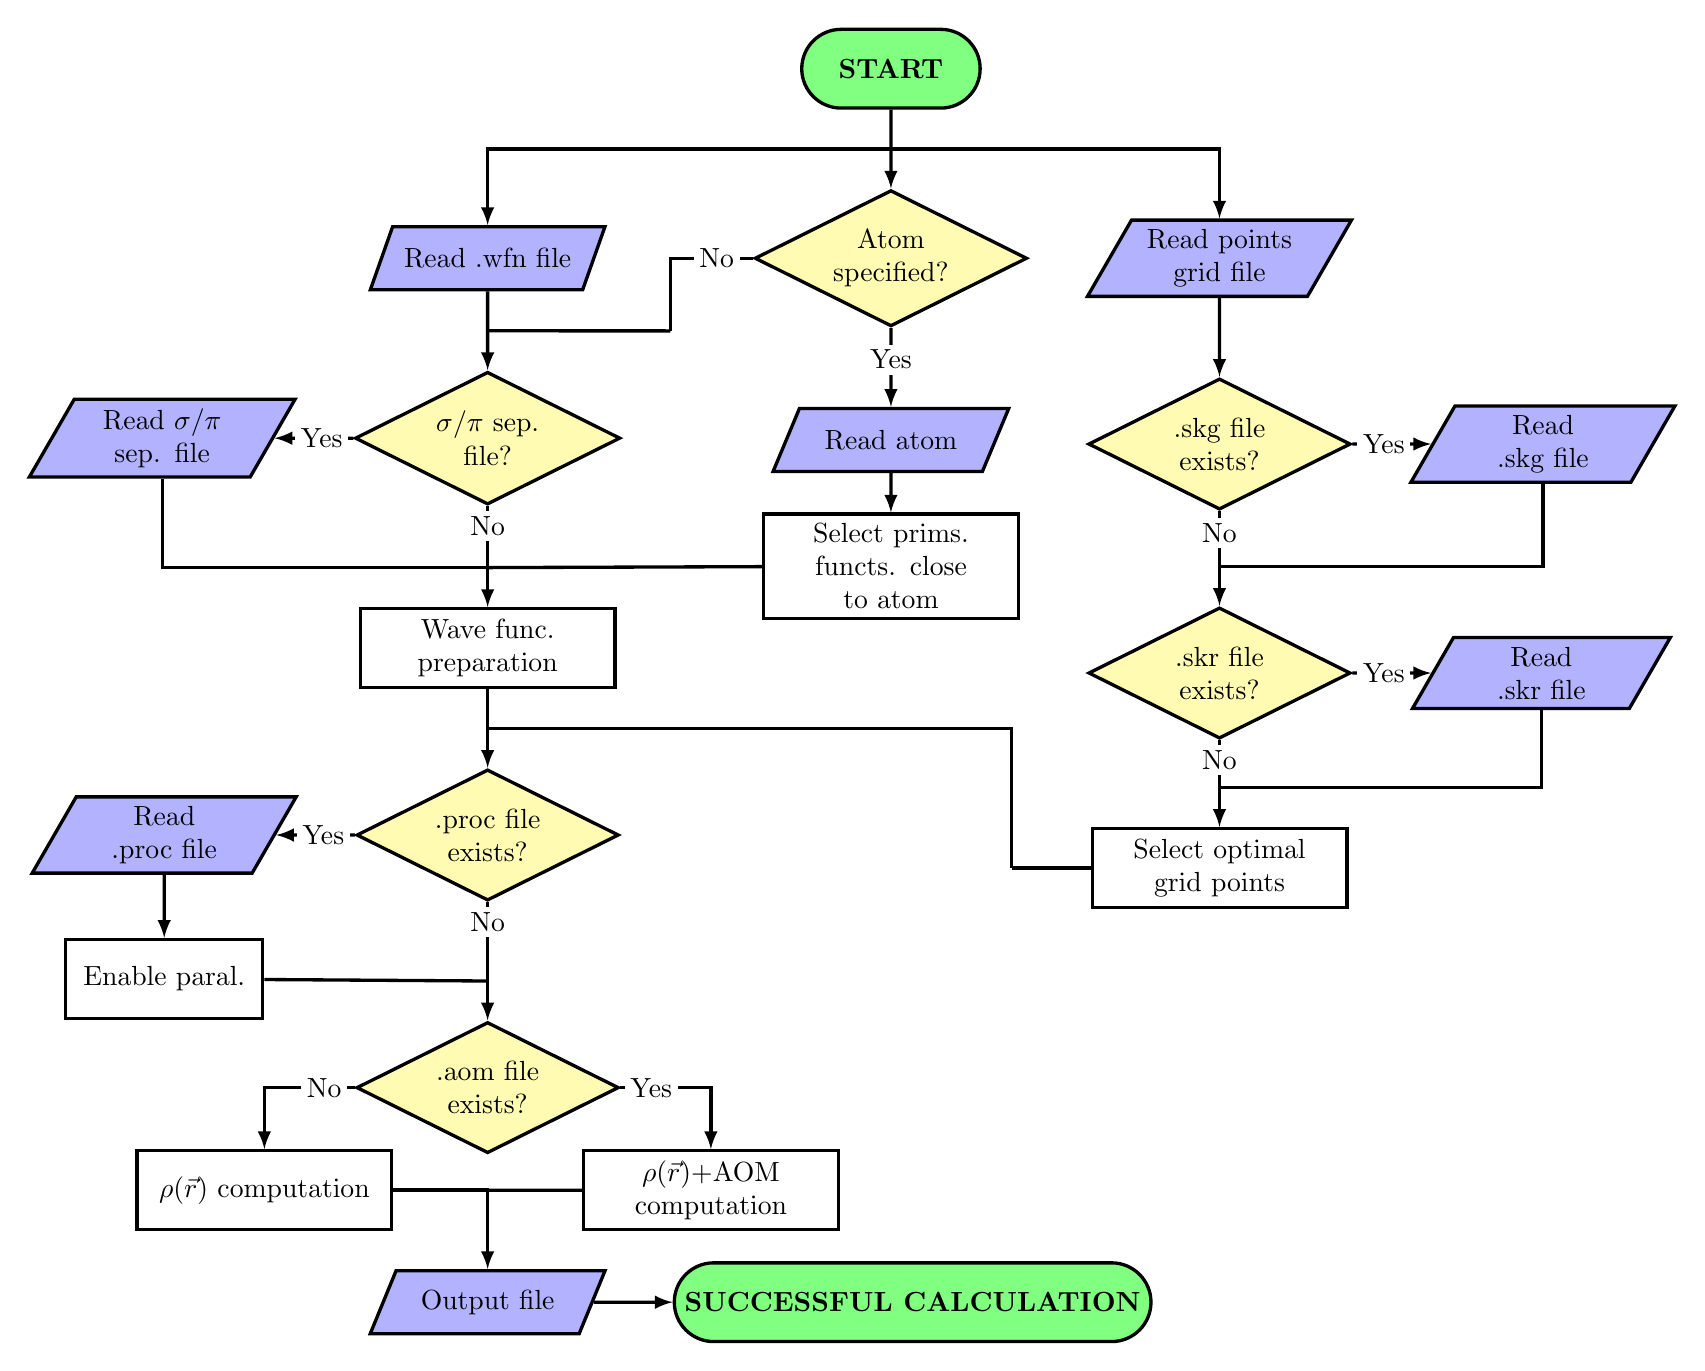
\begin{tikzpicture}[font=\normalsize,very thick,align=center]
		
		% Start block
		\node[
			draw,
			fill=green!50,
			rounded rectangle,
			minimum width=2.5cm,
			minimum height=1cm
		] (start) {\textbf{START}};
		
		\node[coordinate,below=.5cm of start] (ghoststart) {};
		
		% Third argument?
		\node[
			draw,
			diamond,
			aspect=2,
			minimum width=2.cm,
			text width=3cm,
			text centered,
			inner sep=0,
			fill=yellow!30,
			text width=2cm,
			below=.5cm of ghoststart
		] (thirdarg) {Atom specified?};
		
		\node[coordinate,below left=of thirdarg] (ghostthird) at (-1.8cm,-2.33cm) {};

		% Read wfn file		
		\node[
			draw,
			trapezium, 
			trapezium left angle = 60,
			trapezium right angle = 120,
			trapezium stretches,
			minimum width=3.cm,
			minimum height=.8cm,
			fill=blue!30,
			left=2cm of thirdarg
		] (readwfn) {Read .wfn file};
		
		\node[coordinate,below=.5cm of readwfn] (ghostwfn) {};
		
		% Read grid file
		\node[
			draw,
			trapezium, 
			trapezium left angle = 60,
			trapezium right angle = 120,
			trapezium stretches,
			minimum width=3.cm,
			minimum height=.8cm,
			text width=2cm,
			fill=blue!30,
			right=of thirdarg
		] (readgrid) {Read points grid file};
		
		% Read atom grid is centered on
		\node[
			draw,
			trapezium, 
			trapezium left angle = 60,
			trapezium right angle = 120,
			trapezium stretches,
			minimum width=3.cm,
			minimum height=.8cm,
			fill=blue!30,
			below=of thirdarg
		] (readatom) {Read atom};

		% Read atom grid is centered on
		\node[
			draw,
			minimum width=2.5cm,
			minimum height=1cm,
			text width=3cm,
			below=.5cm of readatom
		] (skipprim) {Select prims. functs. close to atom};
		
		% .sg file exists?
		\node[
			draw,
			diamond,
			aspect=2,
			minimum width=2.cm,
			text width=2cm,
			text centered,
			inner sep=0,
			fill=yellow!30,
			below=.5cm of ghostwfn
		] (sigpi) {$\sigma$/$\pi$ sep. file?};
		
		% Read .sg file
		\node[
			draw,
			trapezium, 
			trapezium left angle = 60,
			trapezium right angle = 120,
			trapezium stretches,
			minimum width=3.cm,
			minimum height=.8cm,
			fill=blue!30,
			text width=2cm,
			left=of sigpi
		] (sgread) {Read $\sigma$/$\pi$ sep. file};
		
		\node[coordinate,below=.78cm of sigpi] (ghostsigpi) {};
		
		% wf user settings
		\node[
			draw,
			minimum width=2.5cm,
			minimum height=1cm,
			text width=3cm,
			below=.5cm of ghostsigpi
		] (wfword) {Wave func. preparation};
		
		\node[coordinate,below=.5cm of wfword] (ghostwfword) {};
		
		% .skg file?
		\node[
			draw,
			diamond,
			aspect=2,
			minimum width=2.cm,
			text width=3cm,
			text centered,
			inner sep=0,
			fill=yellow!30,
			text width=2cm,
			below=of readgrid
		] (skg) {.skg file exists?};
		
		% Read .skg file
		\node[
			draw,
			trapezium, 
			trapezium left angle = 60,
			trapezium right angle = 120,
			trapezium stretches,
			minimum width=3.cm,
			minimum height=.8cm,
			fill=blue!30,
			text width=2cm,
			right=of skg
		] (readskg) {Read .skg file};
		
		\node[coordinate,below=.7cm of skg] (ghostskg) {};
		
		% .skr file?
		\node[
			draw,
			diamond,
			aspect=2,
			minimum width=2.cm,
			text width=2cm,
			text centered,
			inner sep=0,
			fill=yellow!30,
			below=.5cm of ghostskg
		] (skr) {.skr file exists?};
		
		% Read .skg file
		\node[
			draw,
			trapezium, 
			trapezium left angle = 60,
			trapezium right angle = 120,
			trapezium stretches,
			minimum width=3.cm,
			minimum height=.8cm,
			fill=blue!30,
			text width=2cm,
			right=of skr
		] (readskr) {Read .skr file};
		
		\node[coordinate,below=.6cm of skr] (ghostskr) {};
		
		% Read .skg file
		\node[
			draw,
			minimum width=2.5cm,
			minimum height=1cm,
			text width=3cm,
			below=.5cm of ghostskr
		] (optgrid) {Select optimal grid points};
		
		\node[coordinate,left=of optgrid] (ghostoptgrid) {};
		
		% .proc file?
		\node[
			draw,
			diamond,
			aspect=2,
			minimum width=2.cm,
			text width=2cm,
			text centered,
			inner sep=0,
			fill=yellow!30,
			below=.5cm of ghostwfword,
		] (proc) {.proc file exists?};
		
		% Read .proc file
		\node[
			draw,
			trapezium, 
			trapezium left angle = 60,
			trapezium right angle = 120,
			trapezium stretches,
			minimum width=3.cm,
			minimum height=.8cm,
			fill=blue!30,
			text width=2cm,
			left=of proc
		] (readproc) {Read .proc file};
		
		\node[
			draw,
			minimum width=2.5cm,
			minimum height=1cm,
			below=.8cm of readproc
		] (paral) {Enable paral.};
		
		\node[coordinate,below=of proc] (ghostproc) {};
		
		% .aom file?
		\node[
			draw,
			diamond,
			aspect=2,
			minimum width=2.cm,
			text width=2cm,
			text centered,
			inner sep=0,
			fill=yellow!30,
			below=.5cm of ghostproc
		] (aom) {.aom file exists?};
		
		% dens calc
		\node[
			draw,
			minimum width=2.5cm,
			minimum height=1cm,
			text width=3cm,
			below left=.5cm of aom
		] (dens) {$\rho(\vec{r})$ computation};
		
		% AOM+dens calc
		\node[
			draw,
			minimum width=2.5cm,
			minimum height=1cm,
			text width=3cm,
			below right=.5cm of aom
		] (aomdens) {$\rho(\vec{r})$+AOM computation};
		
		\node[coordinate,below=.45cm of aom] (ghostaom) {};
		
		% Output file
		\node[
		draw,
			trapezium, 
			trapezium left angle = 60,
			trapezium right angle = 120,
			trapezium stretches,
			minimum width=3.cm,
			minimum height=.8cm,
			fill=blue!30,
			text width=2cm,
			below=of ghostaom
		] (output) {Output file};
		
		% END
		\node[
			draw,
			fill=green!50,
			rounded rectangle,
			minimum width=2.5cm,
			minimum height=1cm,
			right=of output
		] (end) {\textbf{SUCCESSFUL CALCULATION}};
		
		% Arrows
		\draw[-latex]
			(start) 	 	edge 												(thirdarg)
			(readwfn) 	 	edge 												(sigpi)
			(readgrid)		 edge												(skg)
			(wfword)	 	edge												(proc)
			(readproc)		 edge												(paral)
			(dens)	 		 -|													(output)
			(output)	 	edge 												(end)
			(readatom)	 	edge												(skipprim)
		;
		\draw[-latex]
			(ghoststart) 	-| 													(readwfn)
		;
		\draw[-latex]
			(ghoststart) 	-| 													(readgrid)
		;
		\draw
			(ghostthird) 	edge 												(ghostwfn)
			(skipprim)	 	edge 												(ghostsigpi)
			(readskg)	 	|- 													(ghostskg)
			(readskr)	 	|- 													(ghostskr)
			(optgrid)	 	edge 												(ghostoptgrid)
				(ghostoptgrid)	|-												(ghostwfword)
			(sgread)	 	|-													(ghostsigpi)
			(paral)	 	 	edge												(ghostproc)
			(aomdens)	 	edge 												(ghostaom)
		;
		\draw[-latex] 
			(thirdarg)		edge node[pos=0.4,fill=white,inner sep=2pt]{Yes}	(readatom)
			(skg)			edge node[pos=0.4,fill=white,inner sep=2pt]{Yes}	(readskg)
			(skr)			edge node[pos=0.4,fill=white,inner sep=2pt]{Yes}	(readskr)
			(sigpi)			edge node[pos=0.4,fill=white,inner sep=2pt]{Yes}	(sgread)
			(proc)			edge node[pos=0.4,fill=white,inner sep=2pt]{Yes}	(readproc)
			(aom)			 -|	  node[pos=0.17,fill=white,inner sep=2pt]{Yes}	(aomdens)
		;
		\draw
			(thirdarg)		-|	 node[pos=0.22,fill=white,inner sep=2pt]{No}	(ghostthird)
		;
		\draw[-latex] 
			(sigpi)			 edge node[pos=0.2,fill=white,inner sep=2pt]{No}	(wfword)
			(skg)			 edge node[pos=0.23,fill=white,inner sep=2pt]{No}	(skr)
			(skr)			 edge node[pos=0.23,fill=white,inner sep=2pt]{No}	(optgrid)
			(proc)			 edge node[pos=0.17,fill=white,inner sep=2pt]{No}	(aom)
			(aom)			 -|	  node[pos=0.17,fill=white,inner sep=2pt]{No}	(dens)
		;

		% * (start) {START};
		% * (ghoststart);
		% * (thirdarg) {Atom specified?};
		% * (ghostthird) {};
		% * (readwfn) {Read .wfn file};
		% * (ghostwfn) {};
		% * (readgrid) {Read points grid file};
		% * (readatom) {Read atom grid is centered on};
		% * (skipprim) {Skipping primitive function far from atom};
		% * (sigpi) {$\sigma$/$\pi$ sep. file?};
		% * (ghostsigpi) {};
		% * (sgread) {Read $\sigma$/$\pi$ sep. file};
		% * (wfword) {wave func. preparation};
		% * (ghostwfword) {};
		% * (skg) {.skg file exists?};
		% * (readskg) {Read .skg file};
		% * (ghostskg) {};
		% * (skr) {.skr file exists?};
		% * (readskr) {Read .skr file};
		% * (ghostskr) {};
		% * (optgrid) {Select optimal grid points};
		% * (ghostoptgrid) {};
		% * (proc) {.proc file exists?};
		% * (ghostproc) {};
		% * (readproc) {Read .proc file};
		% * (paral) {Enable paral.};
		% * (ghostproc) {};
		% * (aom) {.aom file exists?};
		% * (dens) {$\rho(\vec{r})$ computation};
		% * (aomdens) {$\rho(\vec{r})$+AOM computation};
		% * (ghostaom) {};
		% * (output) {Output file};
		
	\end{tikzpicture}
	
\end{document}